\section{Potential benefits of ray tracing}
Going away from the current rasterization-based rendering pipeline and instead using ray tracing to render the scene has many potential benefits.

\subsection{Better Representation}
In the current representation of each Gaussian, several extra steps are required to guarantee correctness.

\subsection{Polarization Cameras}
Reflections in the scene pose a significant challenge in the field of \gls{nvs}, as it requires the ability to capture view-dependent color.
As discussed earlier, the use of spherical harmonics solves this to some degree, but it comes at a significant memory cost.
Using polarization cameras might prove very useful in this regard, as reflected light has a distinct polarization signature \cite{lingUniversityPhysicsVolume2016}.

\begin{figure}
    \centering
    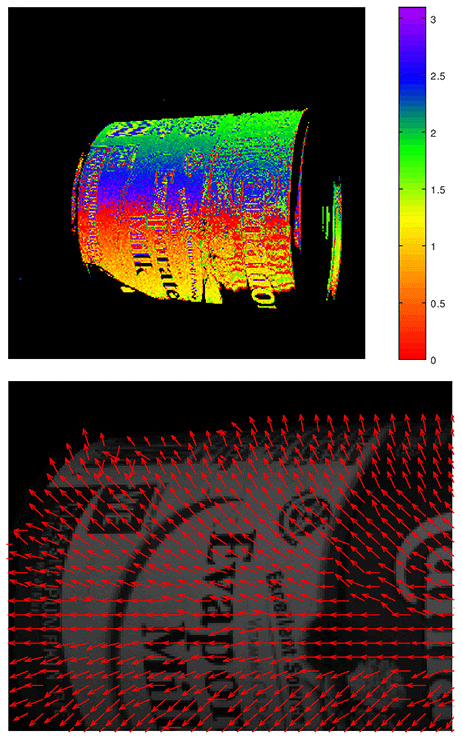
\includegraphics[width=\linewidth]{images/polarization_normals.png}
    \caption{Angle of orientation and estimated surface normals from polarized light \cite{lucidvisionlabs3DDepthSurface2021}}.
    \label{fig:polarization}
\end{figure}


In order to capture view-dependent color from reflections, each Gaussian in the current implementation uses spherical harmonics.
This comes at a memory cost, as 48 out of the 60 parameters of each Gaussian are used to store the spherical harmonics coefficients.
Removing this could lead to a significant reduction in memory usage.

Using polarization cameras it is possible to capture information about both the degree and angle of polariation of each pixel in an image.
A simple way to use this information would be to remove as much reflected light as possible, and partially circumvent the need for view-dependent color.

Another interesting


Another more Potential approach is to use the polarization information to estimate the surface normal of each triangle and perform ray tracing to

As discussed, the main source of view-dependent color is reflections from the environment.
While it probably will have a big, or even detrimental, effect on the performance, it would be interseting to.




\subsection{Code closer to Problem formulation}
There is a significant difference between how the problem is formulated in the paper and how